% A parametrized curve: the interval I, the map alpha, the trace and a tangent vector.
% Build the SVG with ./build.sh (needs latex and dvisvgm, both part of MacTeX).
\def\pgfsysdriver{pgfsys-dvisvgm.def}
\documentclass[tikz,border=6pt]{standalone}
\usepackage{amsmath,amssymb}
\usetikzlibrary{calc}
\definecolor{curve}{HTML}{2563EB}
\definecolor{pt}{HTML}{D97706}
\definecolor{ink}{HTML}{1C1F26}
\definecolor{soft}{HTML}{6B7280}
\begin{document}
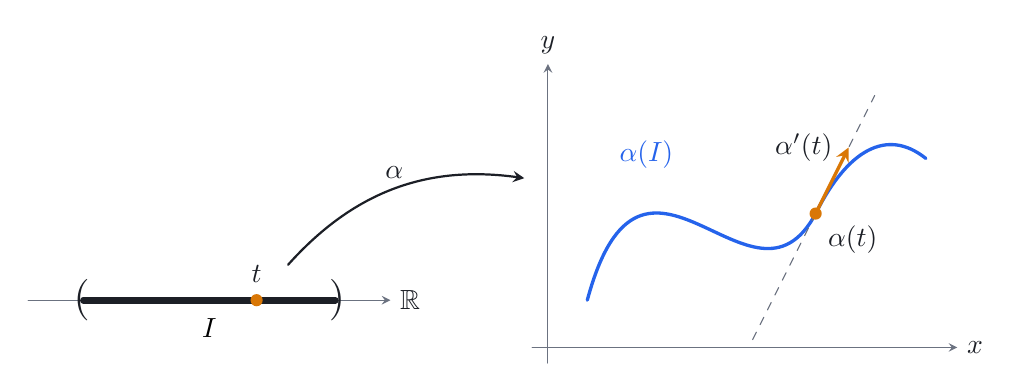
\begin{tikzpicture}[>=stealth, line cap=round, line join=round]
  % the interval I = (a, b) on the real line
  \draw[->, soft] (-0.3,0) -- (4.3,0) node[right, ink] {$\mathbb{R}$};
  \draw[line width=2.4pt, ink] (0.4,0) -- (3.6,0);
  \node[ink, scale=1.5] at (0.38,0.0) {(};
  \node[ink, scale=1.5] at (3.62,0.0) {)};
  \node[below=3pt] at (2.0,0) {$I$};
  \fill[pt] (2.6,0) circle (2.2pt) node[above=3pt, ink] {$t$};

  % the map alpha
  \draw[->, thick, ink] (3.0,0.45) to[bend left=28] node[above, pos=0.5] {$\alpha$} (6.0,1.55);

  % the plane, the trace alpha(I), the point alpha(t) and the tangent vector alpha'(t)
  \begin{scope}[shift={(6.3,-0.6)}]
    \draw[->, soft] (-0.2,0) -- (5.2,0) node[right, ink] {$x$};
    \draw[->, soft] (0,-0.2) -- (0,3.6) node[above, ink] {$y$};
    \draw[very thick, curve] (0.5,0.6) .. controls (1.2,3.2) and (2.6,0.2) .. (3.4,1.7)
                                       .. controls (3.8,2.5) and (4.3,2.8) .. (4.8,2.4);
    \node[curve] at (1.25,2.45) {$\alpha(I)$};
    \coordinate (P) at (3.4,1.7);
    \draw[dashed, soft] ($(P)+(-0.8,-1.6)$) -- ($(P)+(0.75,1.5)$);
    \draw[->, very thick, pt] (P) -- ++(0.42,0.84) node[left=2pt, ink] {$\alpha'(t)$};
    \fill[pt] (P) circle (2.2pt);
    \node[below right=1pt, ink] at (P) {$\alpha(t)$};
  \end{scope}
\end{tikzpicture}
\end{document}
